% -*- program: xelatex -*-
\documentclass[12pt, compress]{beamer}
%\usepackage{listings}

\usepackage{pgfpages}

%\documentclass{article}
%\usepackage{beamerarticle}

%\documentclass[12pt, compress]{beamer} 
%\documentclass[notes=only]{beamer}

\usepackage{fontspec}

\setsansfont{PT Sans}
\setmonofont{PT Mono}

\usepackage{beamerthemesplit}
\usefonttheme[onlymath]{serif}
%\DeclareFontEncoding{T1}
\fontencoding{T1}

%\usepackage[T2A]{fontenc}
%\usepackage[utf8]{inputenc}
\usepackage[russian]{babel}
\usepackage{listings}


\usepackage{amsmath,amssymb,amsthm}
\hypersetup{unicode=true}

\usepackage{color}
\definecolor{mygred}{RGB}{150,0,0} 
\definecolor{mygreen}{RGB}{28,172,0} 
\definecolor{mylilas}{RGB}{170,55,241}
\definecolor{codecolor}{RGB}{0,120,0}
\definecolor{emphcolor}{RGB}{0,0,120}
\definecolor{gray}{RGB}{150,150,150}

\definecolor{light-gray}{gray}{0.95}
\definecolor{light-green}{rgb}{0.93, 1, 0.8}
\definecolor{light-yellow}{rgb}{1,1,0.85}
\definecolor{light-red}{rgb}{0.8, 0.3, 0.3}

\definecolor{dark-blue}{rgb}{0,0,0.6}
\definecolor{dark-red}{rgb}{0.7,0.0,0.0}
\definecolor{dark-green}{RGB}{10,150,0}

\usepackage{pifont}% http://ctan.org/pkg/pifont
\newcommand{\cmark}{\textcolor{green}{\ding{51}}}
\newcommand{\xmark}{\textcolor{red}{\ding{55}}}

\newcommand{\matcode}[1]{ \textcolor{codecolor}{\texttt{#1}}}
\usepackage{graphics,graphicx}
\usepackage{verbatim}
\usepackage{fancyvrb}
\usepackage{booktabs}
%\usepackage{media9}

\usepackage[super]{natbib}
 
\newcommand{\cleartitlepage}[1]{\begin{frame}[plain]\begin{center}\textsc{#1}\end{center}\end{frame}}

\renewcommand{\emph}[1]{\textcolor{emphcolor}{#1}}
\newcommand{\emphb}[1]{\textcolor{emphcolor}{\textbf{#1}}}


\usetheme{CambridgeUS}
\usecolortheme{lily}

\usepackage{tikz}
\usetikzlibrary{positioning} 
\tikzset{cbutton/.style={rectangle,minimum width=10mm,thick,draw=red!50!black!50,
top color=white,bottom color=red!50!black!30}}
\tikzset{mbutton/.style={rectangle,minimum width=10mm,thick,draw=black!20,
top color=white,bottom color=black!30}}


\lstset{basicstyle=\ttfamily\footnotesize,
    language=Python,    
    keepspaces=true,
    extendedchars=true,
    basicstyle={\footnotesize  \color{black}},
    breaklines=true,    
    keywordstyle=\color{blue},
    morekeywords=[2]{1}, keywordstyle=[2]{\color{codecolor}},
    identifierstyle={ \bf \color{black} },
    stringstyle=\color{mylilas},
    commentstyle=\color{mygreen},%
    showstringspaces=false,
    numbers=left,%
    numberstyle={\tiny \color{black}},
    numbersep=7pt, 
    emph=[1]{case,switch,otherwise},emphstyle=[1]\color{blue}, 
    frame=single,    
    rulecolor=\color{red},    
    backgroundcolor=\color{light-gray},
    xleftmargin=0.3cm,
    frame=l,framesep=4pt,framerule=0.5pt,
    showspaces=false,
    escapechar=|
    %lineskip=-0.3pt,
    %emph=[2]{word1,word2}, emphstyle=[2]{style},    
}

\setbeamertemplate{blocks}[rounded][shadow=false]
\setbeamertemplate{navigation symbols}{}

\makeatother
\setbeamertemplate{footline}
{
  \leavevmode%
  \hbox{%
  \begin{beamercolorbox}[wd=.3\paperwidth,ht=2.25ex,dp=1ex,center]{author in head/foot}%
    \usebeamerfont{author in head/foot}\insertshortauthor
  \end{beamercolorbox}%
  \begin{beamercolorbox}[wd=.6\paperwidth,ht=2.25ex,dp=1ex,center]{title in head/foot}%
    \usebeamerfont{title in head/foot}\insertshorttitle
  \end{beamercolorbox}%
  \begin{beamercolorbox}[wd=.1\paperwidth,ht=2.25ex,dp=1ex,center]{date in head/foot}%
    \insertframenumber{} / \inserttotalframenumber\hspace*{1ex}
    %\insertframenumber{} \hspace*{0.1ex}
  \end{beamercolorbox}}%
  \vskip0pt%
}


% define colours
% taken from pickton on Adobe Kuler:
% https://kuler.adobe.com/Some-Kind-Of-Execushares-color-theme-3837185/
 \definecolor{ExecusharesRed}{RGB}{230,37,52}
 \definecolor{ExecusharesBlack}{RGB}{43,40,40}
 \definecolor{ExecusharesBlue}{RGB}{22,190,207}
 \definecolor{ExecusharesWhite}{RGB}{255,255,243}
 \definecolor{ExecusharesGrey}{RGB}{107,110,108}

% \setbeamertemplate{itemize item}{
%  \tikz{
%    \draw[fill=emphcolor,draw=none] (0, 0) rectangle(0.1, 0.1);
%    \draw[fill=emphcolor,draw=none] (0.1, 0.1) rectangle(0.2, 0.2);
%    \draw[fill=emphcolor,draw=none] (0, 0.2) rectangle(0.1, 0.3);
%  }
% }

\AtBeginSection[]{
  \begin{frame}[plain]
  %\vfill  
  \begin{tikzpicture}
  \useasboundingbox (0,0) rectangle(\the\paperwidth,\the\paperheight);  
  \fill[color=mygred]   (-1cm, 3.9cm) rectangle(\the\paperwidth, 5.9cm);
  %\usebeamerfont{title}\insertsectionhead\par%
  %\node[text width=\the\paperwidth,align=center] at (current page.center) {\color{ExecusharesWhite}\Large\textbf{\insertsectionhead}};  
  \node[text width=\the\paperwidth,align=center] at (6cm,4.9cm) {\color{ExecusharesWhite}\Large\textbf{\insertsectionhead}};  
  \end{tikzpicture}
  \end{frame}
}

\setbeamertemplate{headline}{}
\setbeamertemplate{footline}{}

\makeatother
\setbeamertemplate{footline}
{
  \leavevmode%
  \hbox{%  
  \begin{beamercolorbox}[wd=.3\paperwidth,ht=2.25ex,dp=1ex,center]{author in head/foot}%
    \usebeamerfont{author in head/foot}\insertshortauthor
  \end{beamercolorbox}%  
  \begin{beamercolorbox}[wd=.6\paperwidth,ht=2.25ex,dp=1ex,center]{title in head/foot}%
    \usebeamerfont{title in head/foot}\insertshorttitle
  \end{beamercolorbox}%
  \begin{beamercolorbox}[wd=.1\paperwidth,ht=2.25ex,dp=1ex,center]{date in head/foot}%
    \insertframenumber{} \hspace*{1ex}
  \end{beamercolorbox}}%
  \vskip0pt%
}

\setbeamercolor{frametitle}{fg=dark-red,bg=gray!10}
\setbeamerfont{title}{series=\bfseries,parent=structure}
\setbeamerfont{frametitle}{series=\bfseries,parent=structure}

\usepackage{media9}

\definecolor{dark-blue}{rgb}{0,0,0.6}
\definecolor{dark-red}{RGB}{204,0,0}
\definecolor{dark-green}{RGB}{28,172,0}

\lstset{language=Matlab,    
    keepspaces=true,
    extendedchars=true,
    basicstyle={\footnotesize  \color{black}},
    breaklines=true,
    morekeywords={matlab2tikz},
    keywordstyle=\color{blue},
    morekeywords=[2]{1}, keywordstyle=[2]{\color{codecolor}},
    identifierstyle={ \bf \color{black} },
    stringstyle=\color{mylilas},
    commentstyle=\color{mygreen},%
    showstringspaces=false,
    numbers=left,%
    numberstyle={\tiny \color{black}},
    numbersep=7pt,  
    emph=[1]{case,switch,otherwise},emphstyle=[1]\color{blue}, 
    frame=single,    
    %lineskip=-1.0pt,
    %emph=[2]{word1,word2}, emphstyle=[2]{style},    
}

\title{Структурное программирование}
\subtitle{Основы MATLAB}
\author[Кафедра теоретической механики]{Юдинцев В. В.}
\small
\institute{Кафедра теоретической механики}

\begin{document}

{
\usebackgroundtemplate{
\includegraphics[width=\paperwidth,height=\paperheight]{back.png}}
\begin{frame}[plain]
\maketitle
\end{frame}
}

\frame{
\frametitle{Содержание}
\tableofcontents
}

% =============================================================================
%
\section{Циклы}
%
% =============================================================================

\begin{frame}[fragile]{Оператор цикла for}
\begin{lstlisting}
for count = start:step:final
  команды
  команды
end
\end{lstlisting}  
\begin{lstlisting}
a = 0;
for k = 1:10
  a = sin(k*pi)+a;  
end
\end{lstlisting}  
\end{frame}

\begin{frame}[fragile]{Итерации по вектору-строке}
\begin{lstlisting}  
v = [1 2 3];
for i=v
   disp('i:');
   disp(i);
end
\end{lstlisting}  

Результат (тело цикла выполняется 3 раза):
\begin{lstlisting}  
i:
     1

i:
     2

i:
     3
\end{lstlisting}  
\end{frame}


\begin{frame}[fragile]{Итерации по вектору-столбцу}
\begin{lstlisting}  
v = [1; 2; 3];
for i=v
   disp('i:');
   disp(i);
end
\end{lstlisting}  

Результат (тело цикла выполняется 1 раз):
\begin{lstlisting}  
i:
     1
     2 
     3     
\end{lstlisting}  
\end{frame}


\begin{frame}[fragile]{Итерации по матрице}
\begin{lstlisting}  
v = [1 2 3
     4 5 6];
for i=v
    disp('i:');
    disp(i);
end
\end{lstlisting}  
Результат (тело цикла выполняется 3 раза):
\begin{lstlisting}  
i:
     1
     4
i:
     2
     5
i:
     3
     6
\end{lstlisting}       
\end{frame}

\begin{frame}[fragile]{Оператор цикла while}
Общий вид:
\begin{lstlisting}
while условие
  команды
  команды
end    
\end{lstlisting}  
Пример
\begin{lstlisting}
while abs(xErr)<0.001
  x1 = ...;
  x2 = ...;
  xErr = getError(x1,x2);
end    
\end{lstlisting}  
\end{frame}

\begin{frame}[fragile]{Операторы сравнения}
\begin{table}
\begin{tabular}{@{}ll@{}}
\toprule
Функция & Синтаксис \\
\cmidrule{1-2}
Равно & \matcode{х==у} \\
Не равно & \matcode{x\small{$\sim$}=y} \\
Меньше & \matcode{х<у} \\
Больше & \matcode{х>у} \\
Меньше или равно & \matcode{х<=у} \\
Больше или равно & \matcode{х>=у} \\
\bottomrule
\end{tabular}
\end{table}
\end{frame}

\begin{frame}[fragile]{Продолжение выполнения цикла: continue}  
  \begin{itemize}
   \item \matcode{break} -- прерывание цикла.
   \item \matcode{continue} -- продолжение.
  \end{itemize}
\begin{lstlisting}
while условие
  команда 1
  if условие
    команда 2
    continue;
  end
  команда 3      
end    
\end{lstlisting}
``Команда 3'' в седьмой строке не будет исполнена, если условие в строке 3 будет выполнено. 
\end{frame}

\begin{frame}[fragile]{Принудительный выход из блока: break}    
\begin{lstlisting}
while условие
  команда 1
  if условие
    команда 2
    break;
  end
  команда 3      
end
...
\end{lstlisting}
Если условие в строке 3 будет выполнено, то после команды 2 и выхода из цикла, программа продолжит работу со строки 9.
\end{frame}
% =============================================================================
%
\section{Векторизация}
%
% ============================================================================

\begin{frame}[fragile]
\frametitle{Функция linspace}
Функция linspace создает последовательность из $n$ точек в интервале от $a$ до $b$, включая границы
\begin{lstlisting}
>> linspace(5,10,5)

ans =

    5.0000    6.2500    7.5000    8.7500   10.0000
\end{lstlisting}
\end{frame}

\begin{frame}[fragile]{Векторы, как аргументы функции}
Большинство встроенных функций MATLAB корректно обрабатывают аргументы -- векторы (матрицы). 
\begin{lstlisting}
>> sin(1:5)
ans = 
   0.8415    0.9093    0.1411   -0.7568   -0.9589
\end{lstlisting}
\end{frame}

\begin{frame}[fragile]{Векторы, как аргументы функции}
  Вариант 1: функция работает только со скалярным аргументом
\begin{lstlisting}
function f = myfun(x)
  f=exp(-x)*sqrt((x^2+1)/(x^4+0.1))
\end{lstlisting}
Вариант 2: функция адаптирована для векторного аргумента
\begin{lstlisting}
function f = myfun(x)
  f=exp(-x).*sqrt((x.^2+1)./(x.^4+0.1))    
\end{lstlisting}
Вызов функции: \matcode{myfun([0.1 0.2 0.3])}
\end{frame}

\begin{frame}[fragile]
\frametitle{Функция arrayfun}
Функция \matcode{arrayfun} позволяет применить функцию к элементам массива.
\begin{lstlisting}
function f = myfun(x)
  f=exp(-x)*sqrt((x^2+1)/(x^4+0.1))
\end{lstlisting}
Необходимо применить функцию \matcode{myfun} к каждоиу элементу массива $a$:
\begin{lstlisting}
>> a = 1:5

ans  =
       1 2 3 4 5 
\end{lstlisting}
\begin{lstlisting}
>> arrayfun(myfun, a)

ans =
    0.4960    0.0754    0.0175    0.0047    0.0014
\end{lstlisting}
\end{frame}

\begin{frame}[fragile]
\frametitle{Функция arrayfun}
Для функции нескольких аргументов:
\begin{lstlisting}
function res = mean_function(a, b)
  res = (a + b)/2;
\end{lstlisting}
\begin{lstlisting}
>> a = [1 2 3 4];
>> b = [2 3 4 5];
>> arrayfun(mean_function, a, b)

ans =
    1.5000    2.5000    3.5000    4.5000
\end{lstlisting}
\end{frame}

\begin{frame}[fragile]
\frametitle{Векторизация}
Дан массив из 6 векторов расположенных в матрице $3 \times 6$ в столбцах:
\begin{lstlisting}
>> a = [1 2 3 4  5  6  ;
        7 8 9 10 11 12 ;
        1 2 3 4  8  1  ];
\end{lstlisting}     
Модуль векторов можно вычислить, используя оператор цикла:
\begin{lstlisting}
vnorm = zeros( 1, size(a,2) );

for i = 1:size(a,2)
    vnorm(i) = sqrt(a(1,i)^2+a(2,i)^2+a(3,i)^2);
end
\end{lstlisting}
\end{frame}

\begin{frame}[fragile]
\frametitle{Векторизация}
Дан массив из 6 векторов расположенных в матрице $3 \times 6$ в столбцах:
\begin{lstlisting}
>> a = [1 2 3 4  5  6  ;
        7 8 9 10 11 12 ;
        1 2 3 4  8  1  ];
\end{lstlisting}     
Эффективнее использовать встроенные функции:
\begin{lstlisting}
vnorm = sqrt( sum(a.*a, 1) )
\end{lstlisting}
\end{frame}
% =============================================================================
%
\section{Операторы ветвления}
%
% =============================================================================
\begin{frame}[fragile]{Оператор if}
\begin{lstlisting}     
if varA>5
  команды, выполняемые если varA>5      
end
\end{lstlisting}
Больше выбор:
\begin{lstlisting}     
if условие 
  команды      
elseif условие
  команды      
elseif условие
  команды      
else
  команды      
end
\end{lstlisting}
\end{frame}

\begin{frame}[fragile]{Оператор switch}
\begin{lstlisting}
switch varA 
case 1
  команды если varA=1
case 2
  команды если varA=2
case 3
  команды если varA=31
otherwise
  команды 
end      
\end{lstlisting}
\end{frame}

\section{Пример использования векторизации}
%
%
%
\begin{frame}[fragile]{Направления осей $Cx_oy_oz_o$}
\begin{columns} 
\column{0.5\linewidth} 
\begin{center}
 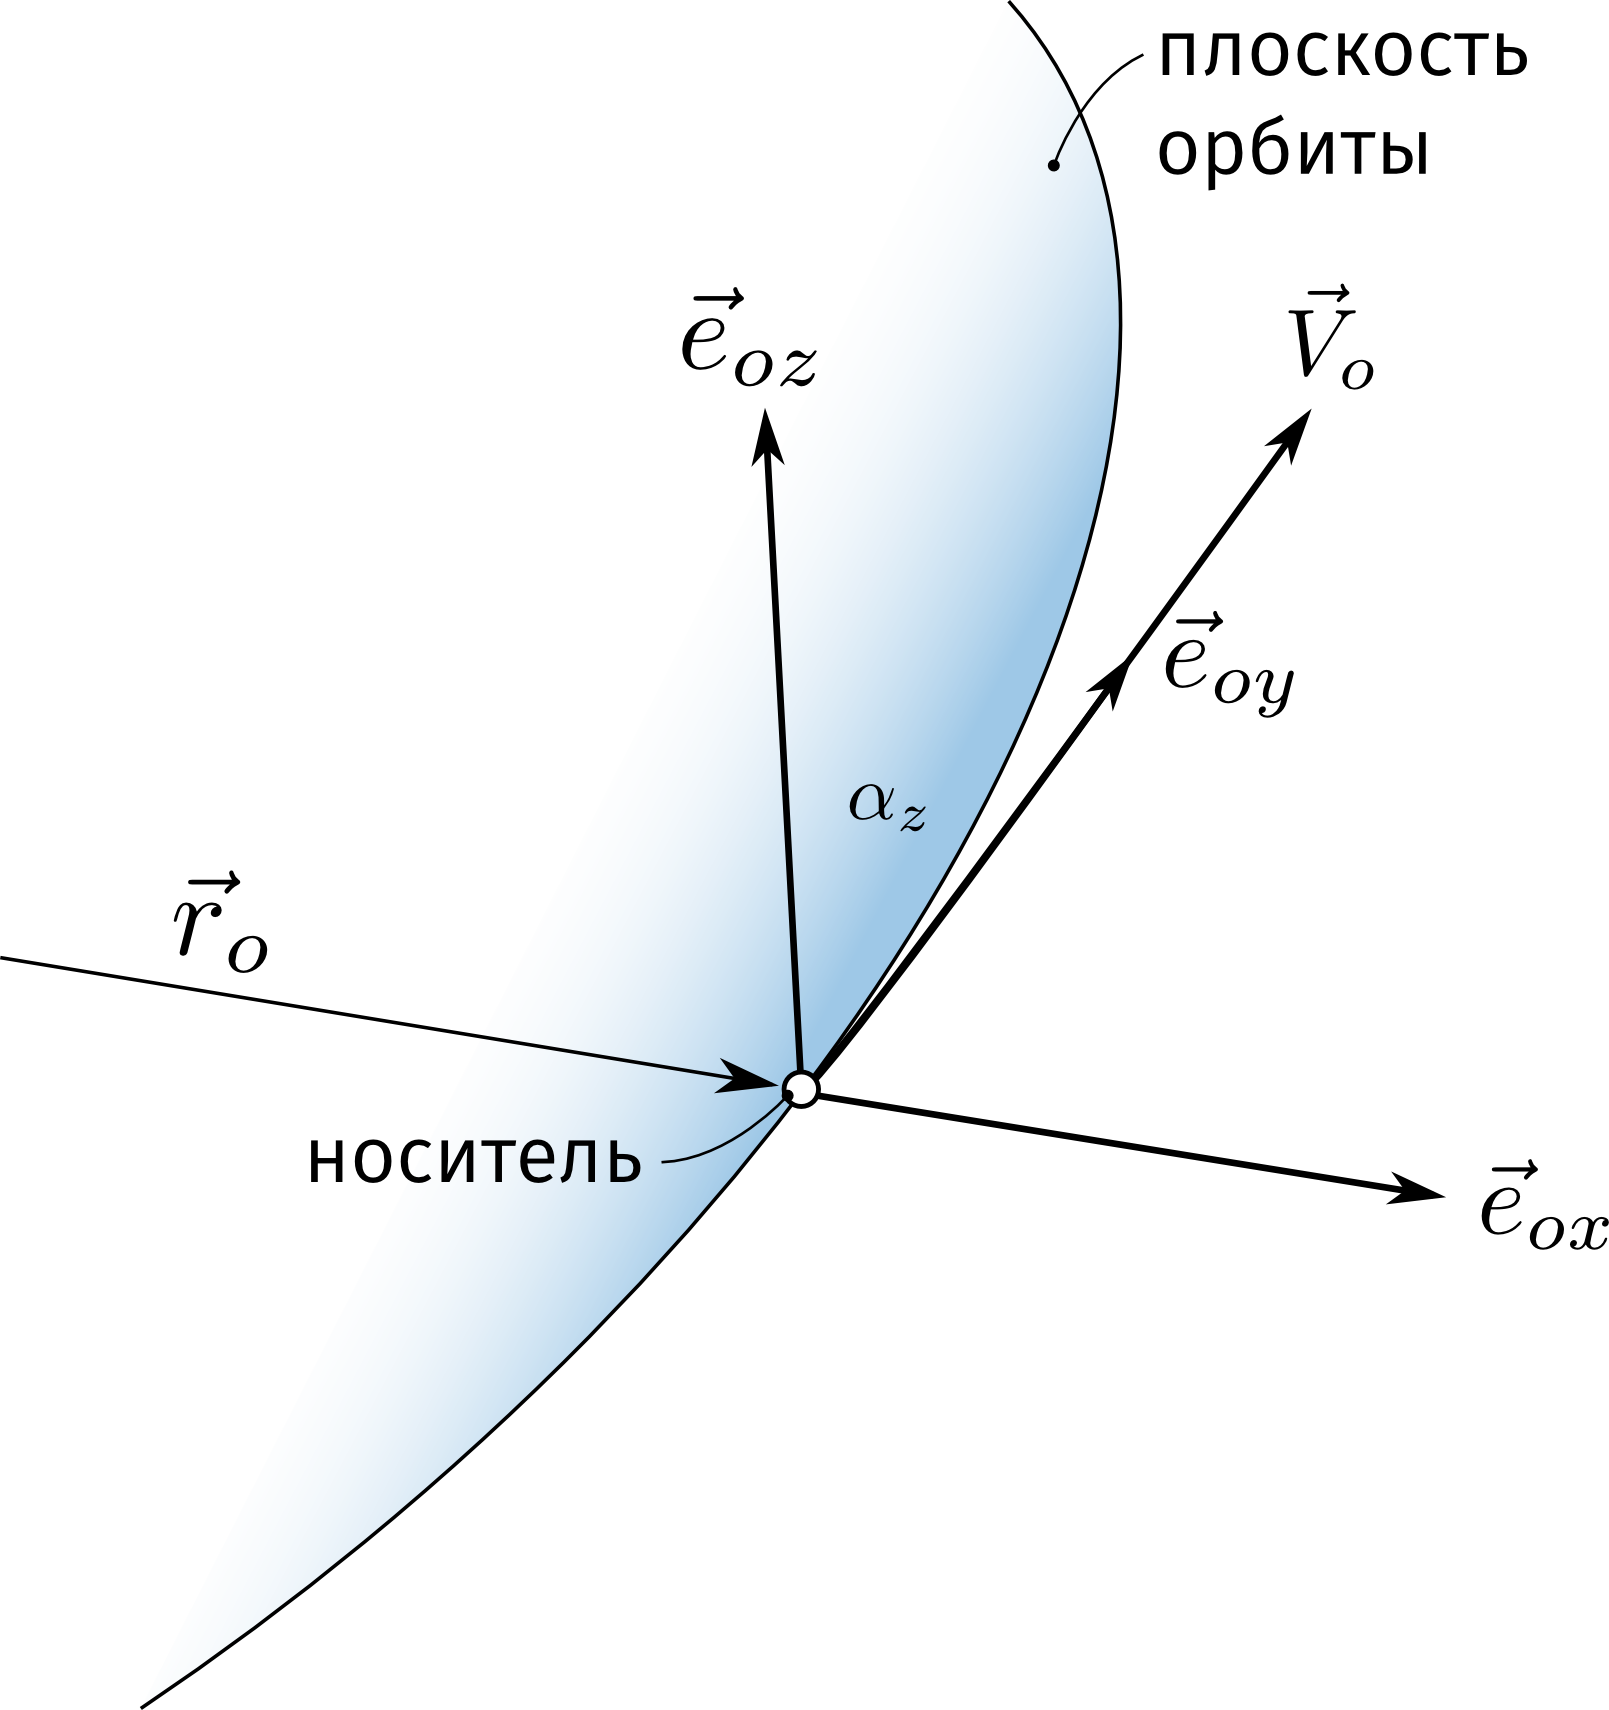
\includegraphics[width=1.0\linewidth]{./orbitalCoordinatesOnly.png} 
\end{center}
\column{0.5\linewidth} 
Единичный вектор радиус-вектора носителя:
$$
\vec e_{ox} = \vec r_0 / r_0.
$$
Единичный вектор нормали к орбите:
$$
\vec e_{oz} = (\vec r_0 \times \vec v_0) / | \vec r_0 \times \vec v_0 |.
$$
Единичный вектор трансверсали:
$$
\vec e_{oy} = (\vec e_{oz} \times \vec e_{ox})/| \vec e_{oz} \times \vec e_{ox} |.
$$
\end{columns}
\end{frame}


\begin{frame}[fragile]{Положение КА относительно носителя}
\begin{columns} 
\column{0.5\linewidth} 
\begin{center}
 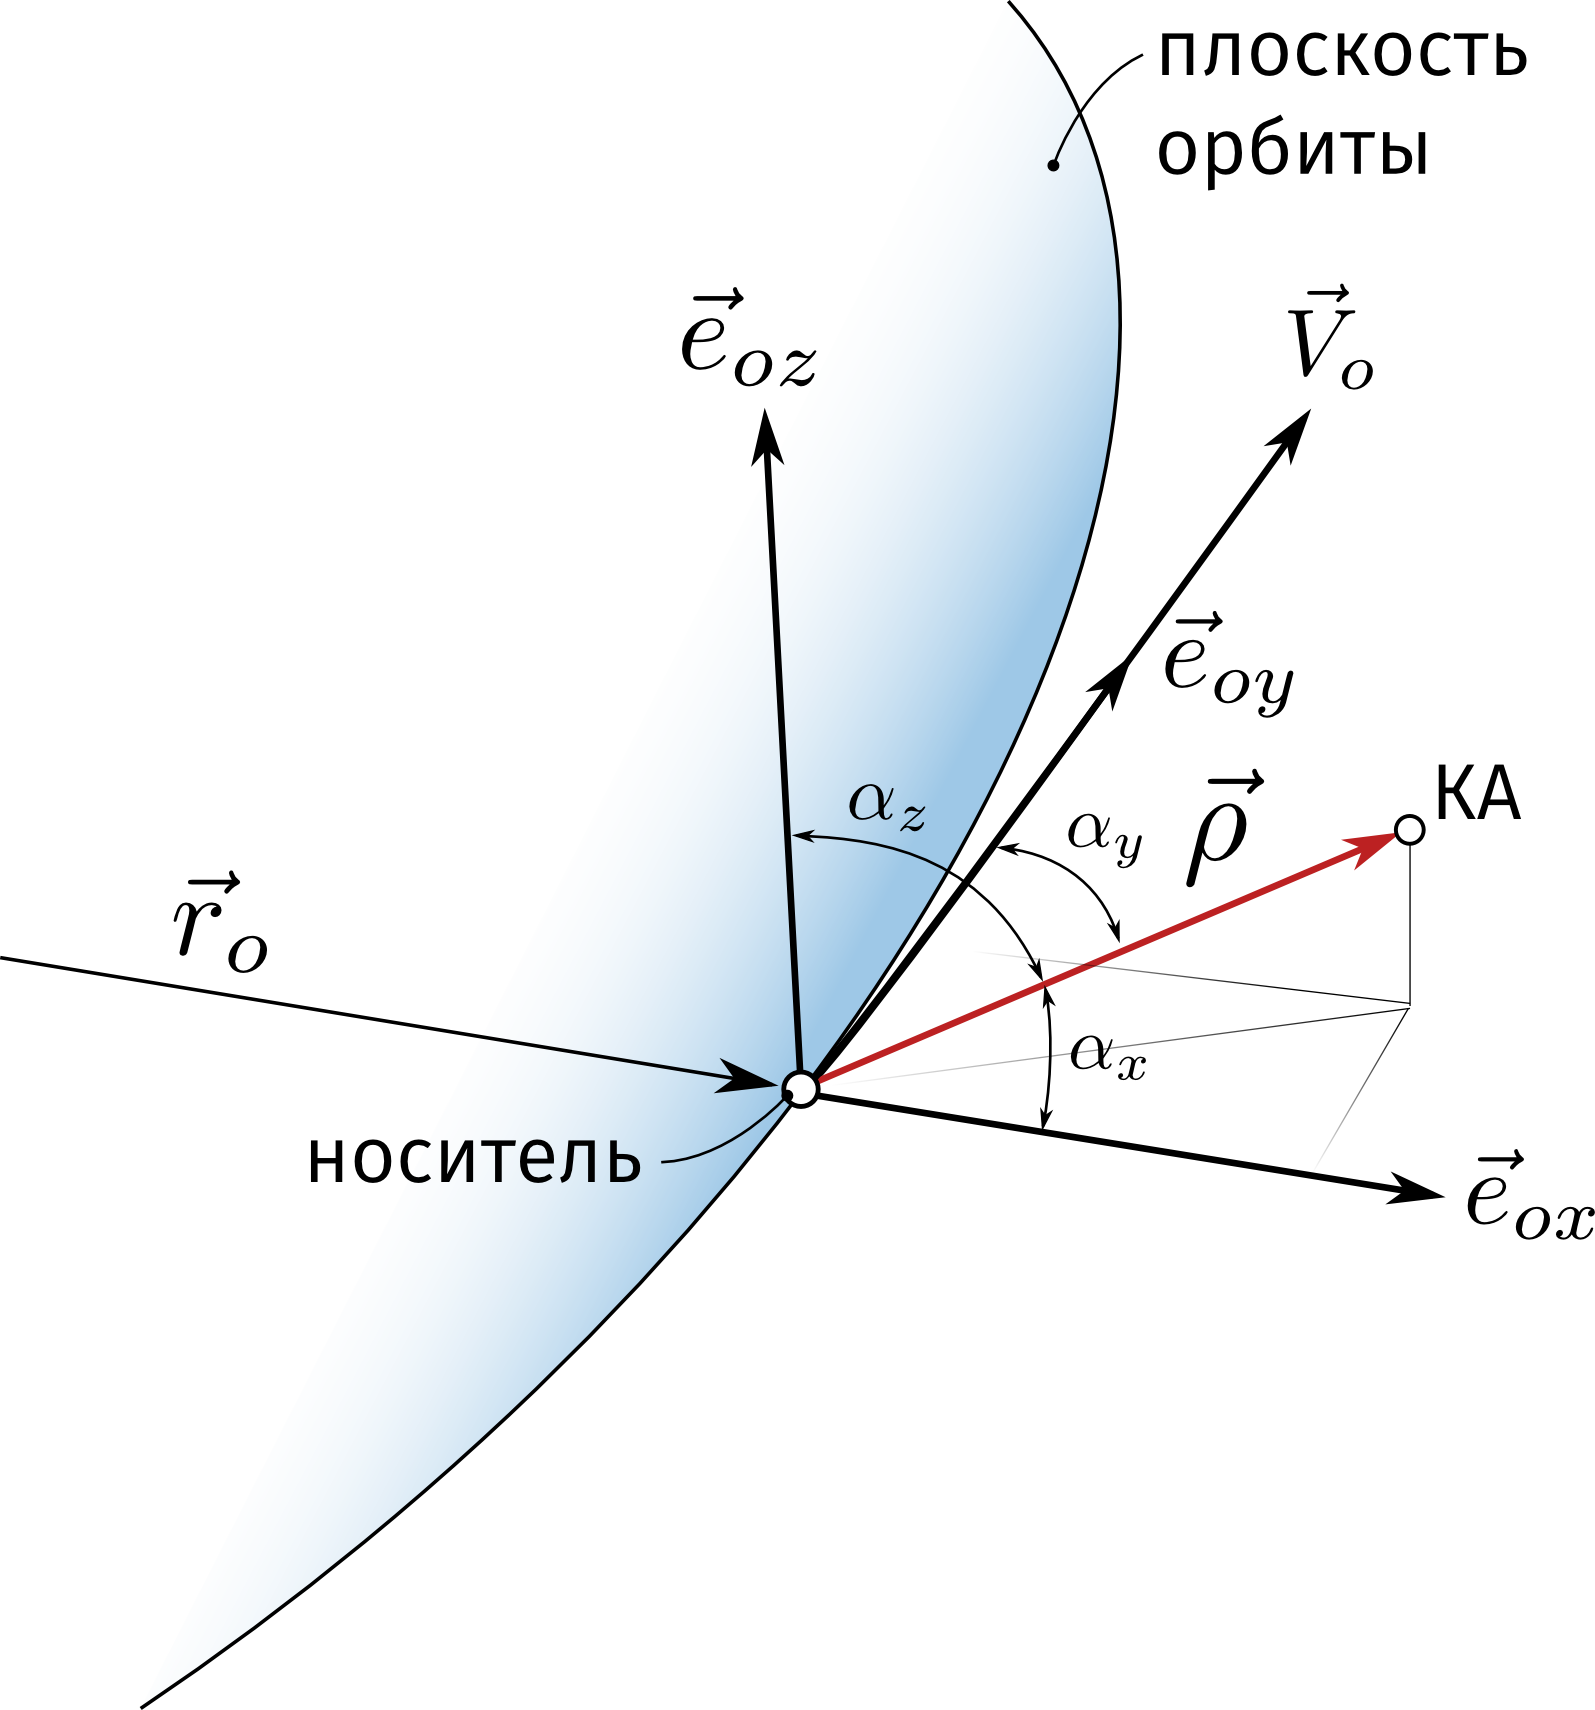
\includegraphics[width=1.0\linewidth]{./orbitalCoordinates.png} 
\end{center}
\column{0.5\linewidth} 
Радиус-вектор положения КА относительно носителя:
$$
\vec \rho = \vec r - \vec r_0
$$
Координаты КА относительно носителя в $Cx_oy_oz_o$:
$$
\begin{aligned}
  & x = \vec \rho \cdot \vec e_{ox}=\vec \rho \cos \alpha_x, \\
  & y = \vec \rho \cdot \vec e_{oy}=\vec \rho \cos \alpha_y, \\
  & z = \vec \rho \cdot \vec e_{oz}=\vec \rho \cos \alpha_z.
\end{aligned}
$$
\end{columns}
\end{frame}


\begin{frame}[fragile]{Вектор относительного положения}
Матрица результатов интегрирования абсолютного движения двух материальных точек:
\begin{lstlisting}
q = 
v1x, v1y, v1z, x1, y1, z1, v2x, v2y, v2z, x2, y2, z2
v1x, v1y, v1z, x1, y1, z1, v2x, v2y, v2z, x2, y2, z2
...
\end{lstlisting}
Координатный столбец вектора положения второй точки относительно первой в проекциях на неподвижную систему координат:
\begin{lstlisting}
rho = q(:,10:12)-q(:,1:3);
\end{lstlisting}
\end{frame}

\begin{frame}[fragile]{Орты орбитальной подвижной системы}
\begin{lstlisting}
q = 
v1x, v1y, v1z, x1, y1, z1, v2x, v2y, v2z, x2, y2, z2
v1x, v1y, v1z, x1, y1, z1, v2x, v2y, v2z, x2, y2, z2
...
\end{lstlisting}
Координатные столбцы единичных векторов орбитальной подвижной системы координат, связанной с первым телом:
\begin{lstlisting}
r = sqrt( sum( q(:,4:6).*q(:,4:6) ,2) );
ex0 = q(:,4:6)./repmat(r,1,3);
\end{lstlisting}
\begin{lstlisting}[firstnumber=last]
v = sqrt( sum( q(:,1:3).*q(:,1:3) ,2) );
ev0 = q(:,4:6)./repmat(v,1,3);
\end{lstlisting}
\end{frame}

\begin{frame}[fragile]{Орты орбитальной подвижной системы}
\begin{lstlisting}
q = 
v1x, v1y, v1z, x1, y1, z1, v2x, v2y, v2z, x2, y2, z2
v1x, v1y, v1z, x1, y1, z1, v2x, v2y, v2z, x2, y2, z2
...
\end{lstlisting}
Единичный вектор нормали к плоскости орбиты:
\begin{lstlisting}
ez0 = cross(ex0,ev0,2);
ez0 = ez0./repmat(sqrt(sum(ez0.*ez0,2)),1,3);
\end{lstlisting}
Единичный вектор трансверсали:
\begin{lstlisting}[firstnumber=last]
ey0 = cross(ez0,er0,2);
ey0 = ey0./repmat(sqrt(sum(ey0.*ey0,2)),1,3);
\end{lstlisting}
\end{frame}



\begin{frame}[fragile]{Относительное положение}
Координатный столбец вектора положения второй точки относительно первой в проекциях на неподвижную систему координат:
\begin{lstlisting}
rho = q(:,10:12)-q(:,1:3);
\end{lstlisting}
Тот же вектор в проекция на оси орбитальной подвижной системы:
\begin{lstlisting}
rho_o = [dot(rho,ex0,2),dot(rho,ey0,2),dot(rho,ez0,2)];
\end{lstlisting}
\end{frame}



% % =============================================================================
% %
% \section{Обработка исключительных ситуаций}
% %
% % =============================================================================
% \frame[containsverbatim]
% {
% \frametitle{Операторы try, catch}
% \begin{lstlisting}
% try
%    C = [A; B];
% catch err   
%    if (strcmp(err.identifier,'MATLAB:catenate:dimensionMismatch'))
%       msg = 'Текст сообщения';
%       error('MATLAB:myCode:dimensions', msg);
%    else
%       rethrow(err);
%    end
% end 
% \end{lstlisting}
% \matcode{ME.identifier} -- идентификатор сообщения об ошибке.

% \matcode{ME.message} -- текст сообщения об ошибке.
% }

% \begin{frame}[fragile]{Предупреждения (warning)}
% \begin{lstlisting}
% function res = fun(a, b)

% if a<0
%   warning('a должен быть больше нуля! a=%s',... num2str(a));
% else
%   ...
% end
% \end{lstlisting}  
% \end{frame}

%
%
\section{Задачи}
%
%
%
% \begin{frame}[fragile]{Конечные разности}
% Дана таблично-заданная функция $y(x)$ на равномерной сетке, например:\\
% \matcode{x=[0.1 0.2 0.3 0.4 0.5 0.6 0.7];}\\
% \matcode{y=[0.3 0.7 0.6 0.2 0.3 0.1 -0.5];}

% Построить матрицу конечных разностей вида
%   $$
%   \begin{pmatrix}
%    y_0 & \Delta y_0 & \Delta^2 y_0 & \ldots & \Delta^n y_0 \\
%    y_1 & \Delta y_1 & \Delta^2 y_1 & \ldots & 0 \\
%    \ldots & \ldots & \ldots & \ldots & 0 \\
%    y_n & \Delta y_n & 0 & \ldots & 0 
%   \end{pmatrix}
%   $$
%   где $\Delta y_0 = y_1 - y_0, \, \Delta^2 y_0 = \Delta y_1 - \Delta y_0, \ldots$
% \end{frame}
 
% \begin{frame}[fragile]{Интервалы возрастания и убывания функции}
% \only<1>{
% Дана таблично-заданная функция $y(x)$:\\  
% \matcode{x=(0.12 0.20 0.41 0.60 0.74 0.82  0.89);}  
% \matcode{y=(0.30 0.70 0.61 0.20 0.31 0.10 -0.50);}  
% }

% Найти интервалы на которых функция убывает и интервалы на которых функция возрастает
% $$
%   r_{inc} = 
%     \begin{bmatrix} 
%     a_1 & b_1 \\ a_2 & b_2 \\ \ldots & \ldots \\ a_n & b_n 
%     \end{bmatrix}, \quad
%   r_{dec} = 
%     \begin{bmatrix} 
%     c_1 & d_1 \\ c_2 & d_2 \\ \ldots & \ldots \\ c_m & d_m 
%     \end{bmatrix}
% $$  
% \only<2>{Функция должна принимать или два аргумента \matcode{x} и \matcode{y} или один аргумент -- матрицу \matcode{xy} в в первом столбце (или в строке) которой находятся значния \matcode{x}, во втором столбце (или в строке) -- значения функции \matcode{y}.
% }
% \end{frame}

\begin{frame}[fragile]{Игра ``Жизнь'' (автор Дж. Конвей)}  
  \begin{enumerate}
   \item Дано бесконечное поле на плоскости, разбитое на квадратные ячейки.
   \item Каждая ячейка может быть пустой или занятой клеткой.
   \item Клетка умирает если вокруг неё меньше 2 или больше 3 соседей (занято меньше 2 или больше 3 смежных ячеек).
   \item Клетка рождается в пустой ячейке если вокруг неё ровно 3 соседа.
   \item Рождение и смерть клеток происходит одновременно.
  \end{enumerate}  
\end{frame}

\begin{frame}[fragile]{Глайдер}  
  \only<1>{
  \begin{center}
  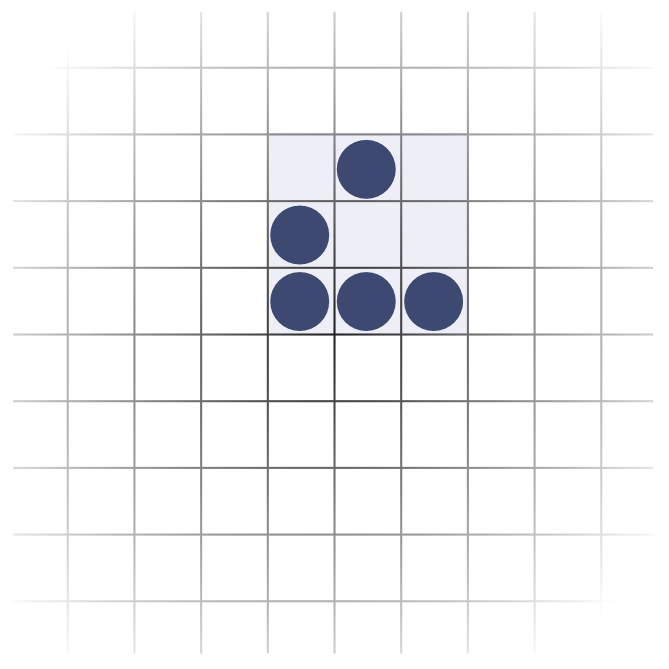
\includegraphics[width=0.6\linewidth]{./life_glider_1.png}  
  \end{center}
  }
  \only<2>{
  \begin{center}
  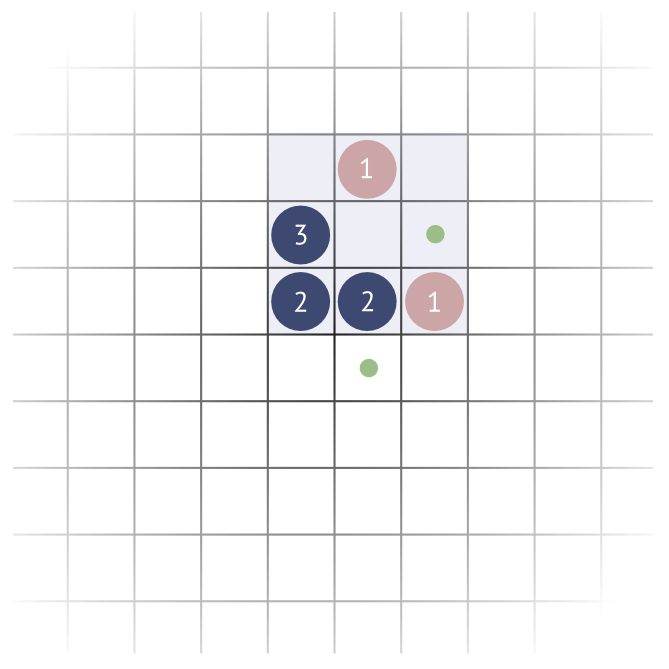
\includegraphics[width=0.6\linewidth]{./life_glider_2.png}  
  \end{center}
  }
  \only<3>{
  \begin{center}
  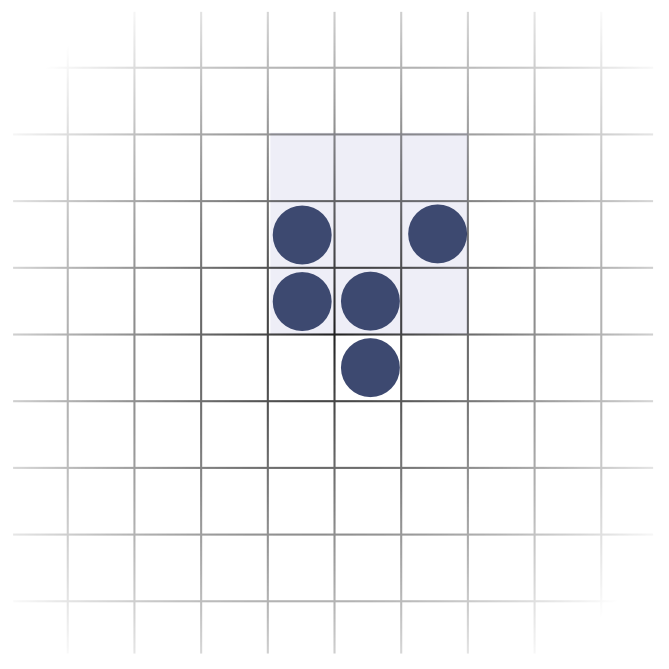
\includegraphics[width=0.6\linewidth]{./life_glider_3.png}  
  \end{center}
  }
  \only<4>{
  \begin{center}
  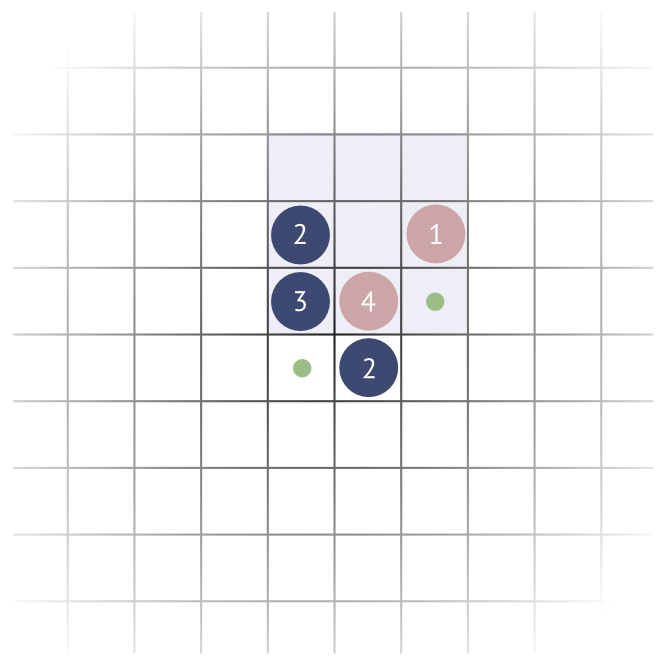
\includegraphics[width=0.6\linewidth]{./life_glider_4.png}  
  \end{center}
  }
  \only<5>{
  \begin{center}
  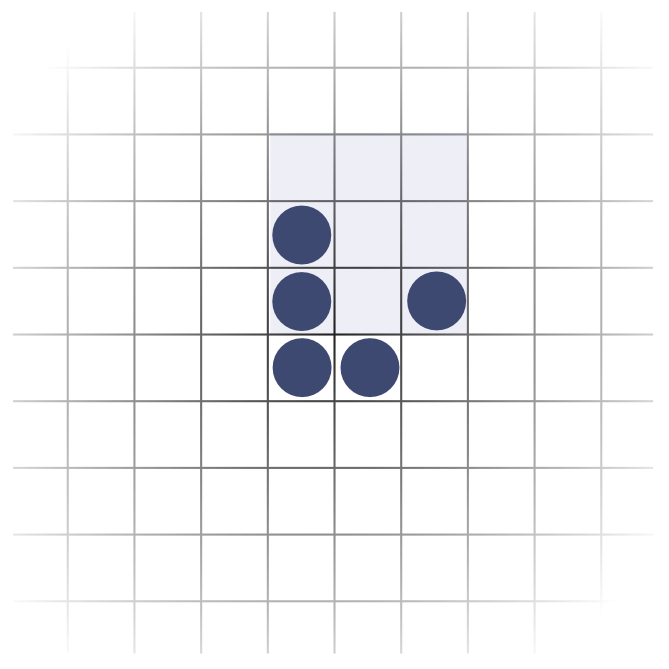
\includegraphics[width=0.6\linewidth]{./life_glider_5.png}  
  \end{center}
  }
  \only<6>{
  \begin{center}
  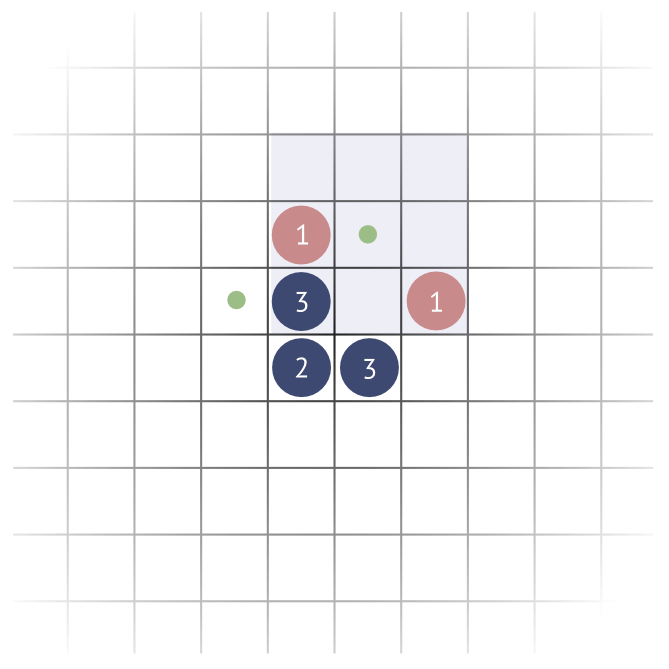
\includegraphics[width=0.6\linewidth]{./life_glider_6.png}  
  \end{center}
  }
  \only<7>{
  \begin{center}
  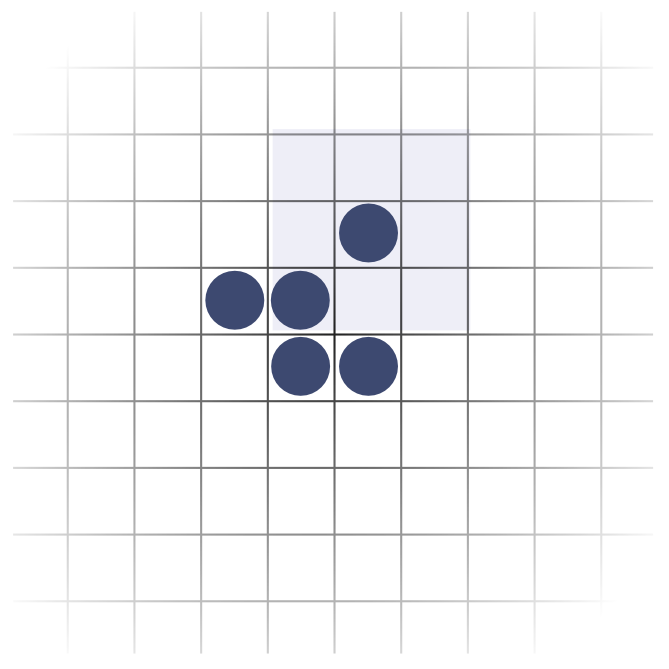
\includegraphics[width=0.6\linewidth]{./life_glider_7.png}  
  \end{center}
  }
  \only<8>{
  \begin{center}
  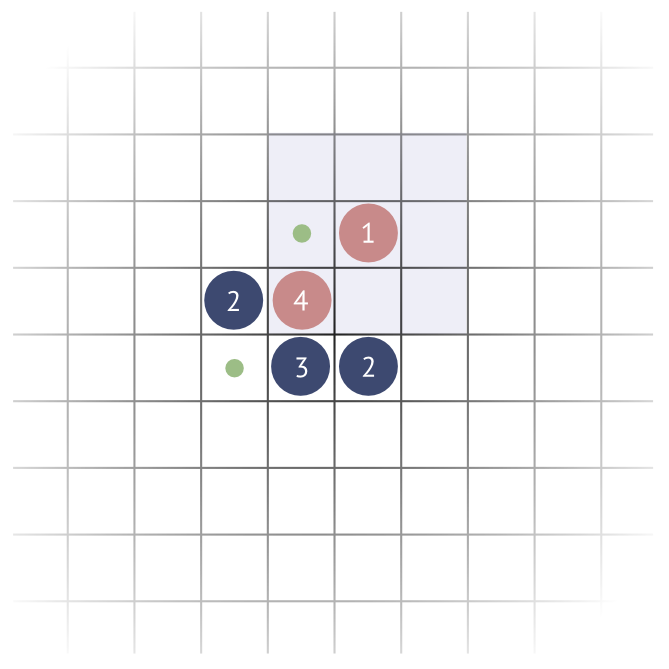
\includegraphics[width=0.6\linewidth]{./life_glider_8.png}  
  \end{center}
  }
  \only<9>{
  \begin{center}
  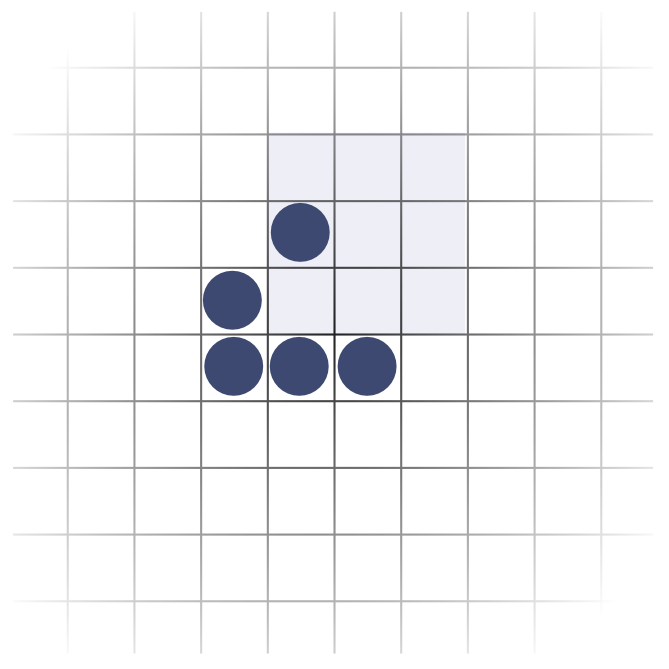
\includegraphics[width=0.6\linewidth]{./life_glider_9.png}  
  \end{center}
  }
\end{frame}


\begin{frame}{}
 \begin{center}
 \includemedia[
   width=0.7\linewidth,height=0.525\linewidth,
   activate=pageopen,
   addresource=Life.mp4,
   flashvars={src=Life.mp4&autohide=1}
 ]{}{APlayer.swf}
 \end{center}
\end{frame}


\begin{frame}[fragile]{Задание}  
\begin{enumerate}
   \item Напишите программу игры ``Жизнь'' на бесконечном поле.
   \item Напишите программу игры ``Жизнь'' на торе (замкнутое пространство).
\end{enumerate}     
\begin{columns}
\column{0.5\linewidth}
   \begin{center}
    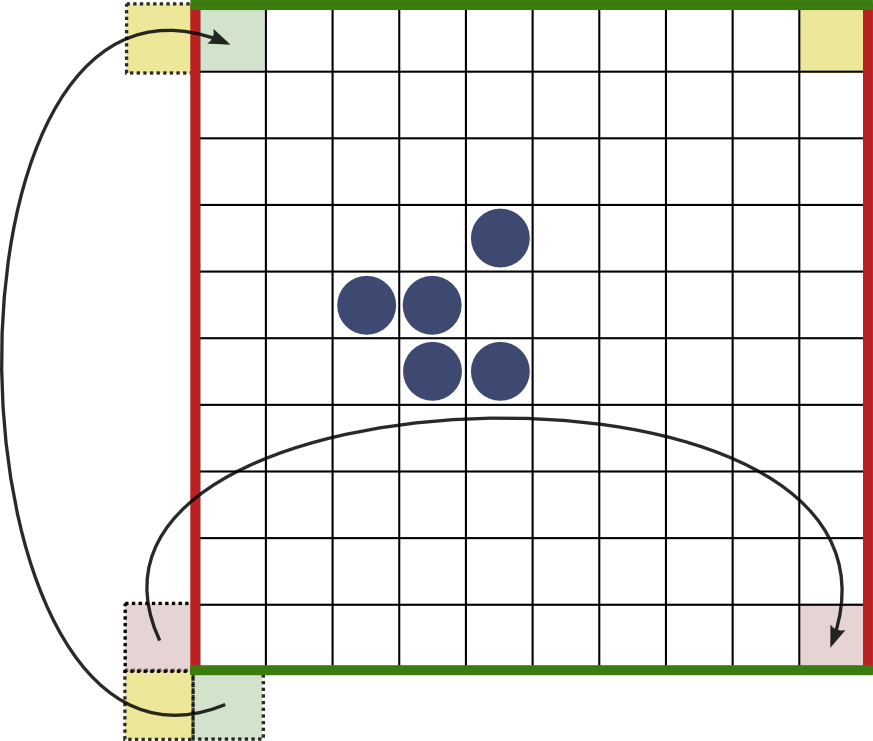
\includegraphics[width=1\linewidth]{./life_tor.png}  
   \end{center}
\column{0.5\linewidth} 
   \begin{center}
    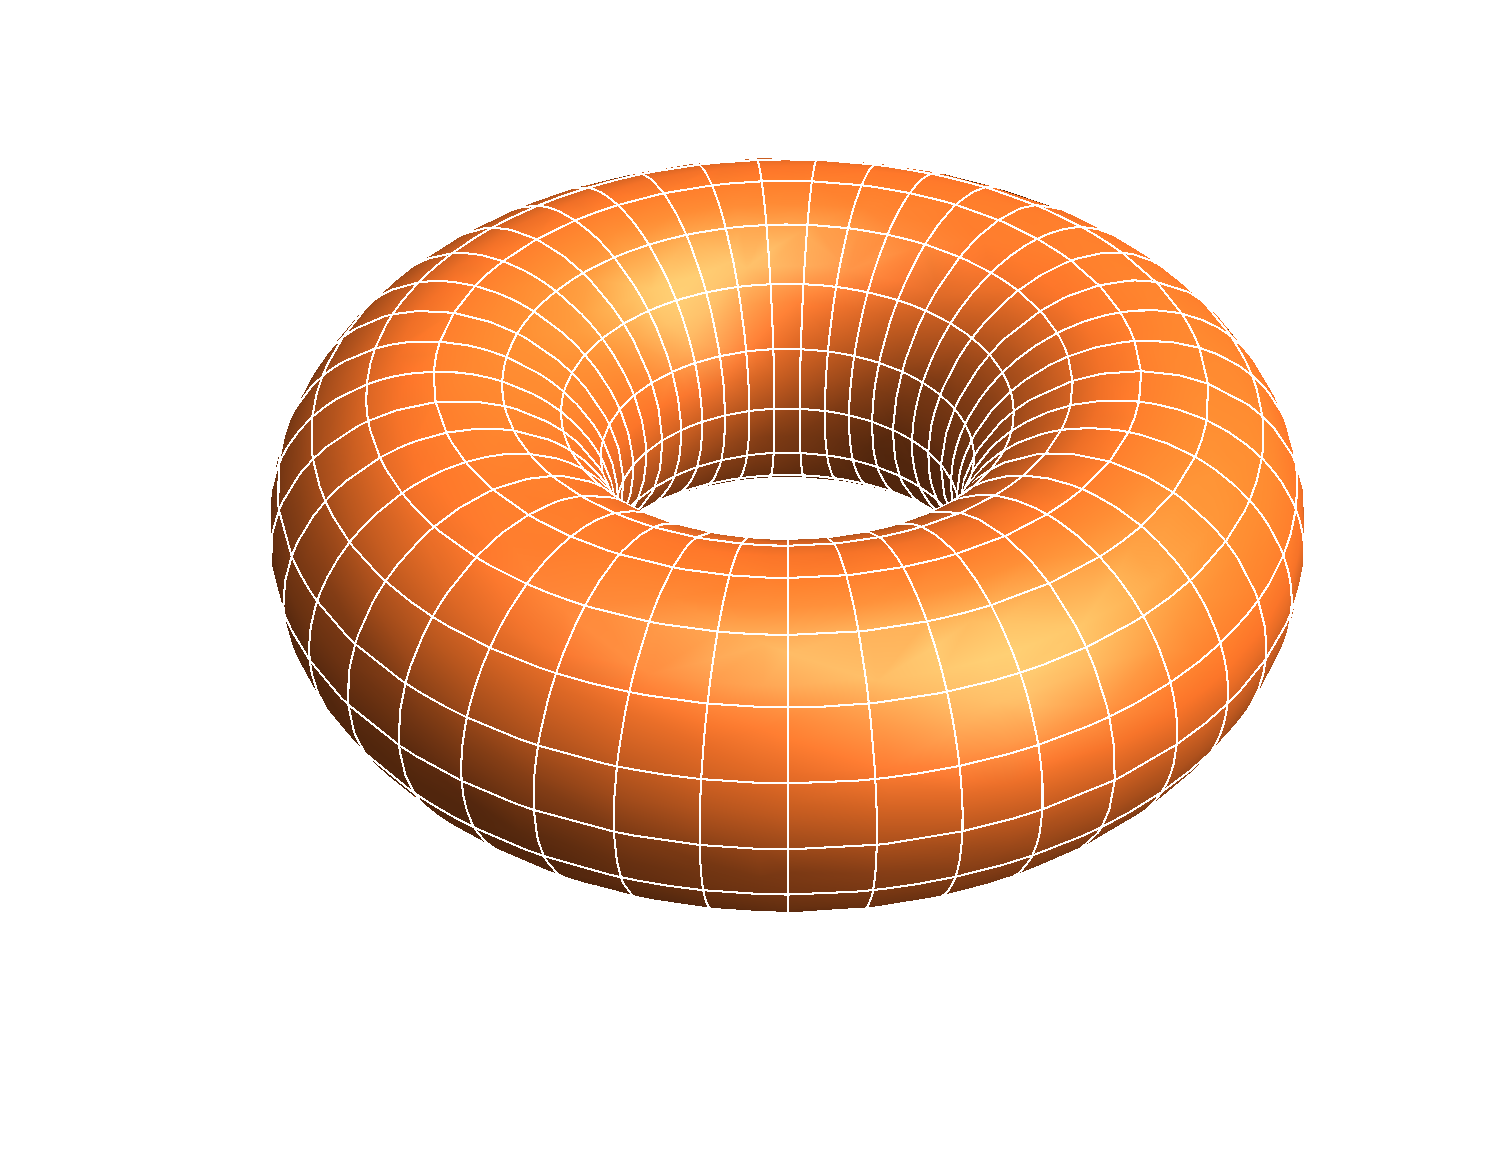
\includegraphics[width=1\linewidth]{./torus.png}  
   \end{center}
\end{columns}
\end{frame}

\begin{frame}[c,fragile]
\frametitle{Типы данных}
Колония клеток (список клеток) задаётся матрицей, состоящей из двух столбцов. Каждая строка матрицы — это пара координат клетки:
$$
  \emph{\text{colony}} = \begin{bmatrix}1 & 1 \\ 2 & 1 \\ 3 & 1 \\ 3 & 2 \\ 2 & 3 \end{bmatrix}
$$  
\begin{lstlisting}
colony = [1, 1; 2, 1; 3, 1; 3, 2; 2, 3];
\end{lstlisting}
Одна клетка задаётся матрицей-строкой из двух элементов — координат клетки:
\begin{lstlisting}
cell = [1, 1];
\end{lstlisting}
\end{frame}


\begin{frame}[fragile]{\emph{Функция} cell\_in\_colony.m}
\begin{lstlisting}
function res = cell_in_colony(cell, colony)  
    ...
\end{lstlisting}     
Аргументы функции:
\begin{itemize}
  \item cell — строка с двумя координатами клетки (x, y) 
  \item colony — матрица $n \times 2$ (два столбца) с координатами клеток колонии
\end{itemize}

Результат работы функции:
\begin{itemize}
  \item 1 — клетка принадлежит колонии
  \item 0 — клетка не принадлежит колонии
\end{itemize}
\end{frame} 


\begin{frame}[t,fragile]
\frametitle{\emph{Функция} get\_neighbours\_cells.m}
\only<1>{
Функция для клетки с координатами \matcode{cell} определяет список координат, граничащих клеток (пустых или занятых):
}
\begin{lstlisting}  
function neighbours = get_neighbours_cells(cell)  
    ...
\end{lstlisting}  
\only<1>{
\begin{center}
\begin{tikzpicture}
[
  box/.style={rectangle,draw=gray,thin, minimum size=3.0cm},
  boxw/.style={rectangle,draw=gray,thin, minimum size=1.0cm},
]
\node[box,fill=light-green] at (2.5,2.5){};  
\draw[step=1cm,color=gray] (0,0) grid (5, 5);
\node at (2.5,1.5) {0,-1};
\node at (3.5,1.5) {1,-1};
\node at (1.5,1.5) {-1,-1};
\node at (3.5,2.5) {1,0};
\node at (1.5,2.5) {-1,0};
\node[boxw,fill=white] at (2.5,2.5){};  
\node at (2.5,2.5) {x,y};
\node at (2.5,3.5) {0,1};
\node at (3.5,3.5) {1,1};
\node at (1.5,3.5) {-1,1};

\node[box,fill=light-green] at (8.5,2.5){};  
\draw[step=1cm,color=gray] (6,0) grid (11, 5);
\node at (7.5,1.7) {x-1};
\node at (7.5,1.3) {y-1};
\node at (8.5,1.7) {x};
\node at (8.5,1.3) {y-1};
\node at (9.5,1.7) {x+1};
\node at (9.5,1.3) {y-1};
\node at (7.5,2.7) {x-1};
\node at (7.5,2.3) {y};
\node[boxw,fill=white] at (8.5,2.5){};  
\node at (8.5,2.5) {x,y};
\node at (9.5,2.7) {x+1};
\node at (9.5,2.3) {y};
\node at (7.5,3.7) {x-1};
\node at (7.5,3.3) {y+1};
\node at (8.5,3.7) {x};
\node at (8.5,3.3) {y+1};
\node at (9.5,3.7) {x+1};
\node at (9.5,3.3) {y+1};
\end{tikzpicture}
\end{center}
}
\end{frame}


\begin{frame}[c,fragile]
\frametitle{\emph{Функция} count\_cell\_neighbours.m}
Функция определяет количество соседей у клетки \matcode{cell} в колонии \matcode{colony}:
\begin{lstlisting}
function count = count_cell_neighbours(cell, colony)  
  ...
\end{lstlisting}
\begin{enumerate}
  \item Определяется список координат клеток-соседей (пустых или занятых).
  \item Для если клетка из этого списка занята (принадлежит колонии), то счётчик соседей клетки \matcode{cell} увеличивается на единицу.
\end{enumerate}
\end{frame}


\begin{frame}[c,fragile]
\frametitle{\emph{Функция} get\_colony\_area.m}
Функция возвращает списко клеток, принадлежащих и граничащих с колонией.
\begin{lstlisting}
function cells = get_colony_area(colony)
  ...
\end{lstlisting}
\begin{center}
\begin{tikzpicture}
[
  box/.style={rectangle,draw=gray,thin, minimum size=0.5cm},
]
\foreach \x in {0,0.5,...,3}{
    \foreach \y in {-0.5,0,...,3.0}
        \node[box] at (\x,\y){};
}
\node[box,fill=dark-red] at (1.0,1.0){};  
\node[box,fill=dark-red] at (1.5,1.0){};  
\node[box,fill=dark-red] at (2.0,1.0){};  
\node[box,fill=dark-red] at (2.0,1.5){};  
\node[box,fill=dark-red] at (1.5,2.0){};  
\node[box,fill=light-green] at (1.0,2.0){};  
\node[box,fill=light-green] at (1.0,2.5){};  
\node[box,fill=light-green] at (1.5,2.5){};  
\node[box,fill=light-green] at (2.0,2.5){};  
\node[box,fill=light-green] at (2.0,2.0){};  
\node[box,fill=light-green] at (2.5,2.0){};  
\node[box,fill=light-green] at (2.5,1.5){};  
\node[box,fill=light-green] at (2.5,1.0){};  
\node[box,fill=light-green] at (2.5,0.5){};  
\node[box,fill=light-green] at (2.0,0.5){};  
\node[box,fill=light-green] at (1.5,0.5){};  
\node[box,fill=light-green] at (1.0,0.5){};  
\node[box,fill=light-green] at (0.5,0.5){};  
\node[box,fill=light-green] at (0.5,1.0){};  
\node[box,fill=light-green] at (0.5,1.5){};  
\node[box,fill=light-green] at (1.0,1.5){};  
\node[box,fill=light-green] at (1.5,1.5){};  

\node[box,fill=light-green] at (4.2,1.5){};  
\node[text width=6.5cm,anchor=west] at (4.5,1.5){Клетки, граничащие с колонией};  
\node[box,fill=dark-red] at (4.2,0.7){};  
\node[text width=6.5cm,anchor=west] at (4.5,0.7){Клетки, принадлежащие колонии};  
\end{tikzpicture}
\end{center}
\end{frame}

\begin{frame}[c,fragile]
\frametitle{\emph{Функция} next\_generation.m}
Функция возвращает матрицу координат клеток следующего поколения для колонии \matcode{colony}:
\begin{lstlisting}
function next_gen = next_generation(colony)
  ...
\end{lstlisting}
Пример работы функции
\begin{lstlisting}
colony = [1, 1; 2, 1; 3, 1; 3, 2; 2, 3];
colony = next_generation(colony);
colony =

   1   2
   2   0
   2   1
   3   1
   3   2
\end{lstlisting}
\end{frame}


\end{document}
